\chapter{Results and Empirical Evaluation}
\label{ch:results}

This chapter presents the empirical evaluation of HalDetect across controlled laboratory benchmarks, open generative road tests, and comparative ablation studies. Following the inside-out experimental formulation, each section presents a concrete finding substantiated by measured quantitative metrics, exact confidence intervals, and paired statistical significance tests.

% ******************************************************************************
\section{Track 1: Master 4-Way Paradigm Benchmark}
\label{sec:track1_results}
% ******************************************************************************

The primary performance hypothesis investigates whether decomposing claims into typed modalities and verifying them through specialized neuro-symbolic arithmetic and knowledge graph engines outperforms monolithic neural baselines. We evaluate all architectures on the Master Benchmark Corpus ($N = 1{,}005$, containing 543 gold \texttt{TRUE}, 433 gold \texttt{FALSE}, and 29 gold \texttt{UNVERIFIABLE} assertions across five distinct modalities).



Structured modalities (Quantitative, Temporal, Entity-Attribute, and Citation) demonstrate near-zero error rates ($\le 2.5\%$). Factual discrepancies in numerical parameters and academic citations are resolved deterministically, while neural NLI is reserved strictly for open relational text.

% ******************************************************************************
\section{In-Depth Forensic Case Studies Across Modalities}
\label{sec:forensic_case_studies}
% ******************************************************************************

To provide granular qualitative insight into how HalDetect operates, we examine five representative case studies spanning each verification modality:

\subsection{Case Study 1: Quantitative Hardware Transistor Contradiction}
\begin{itemize}
    \item \textbf{Generated Assertion:} \textit{"The Apple M3 Max processor integrates 40 million transistors."}
    \item \textbf{Atomized Tuple:} $\langle \text{Apple M3 Max}, \text{transistor\_count}, 40\times 10^6, \text{None}, \text{None} \rangle$.
    \item \textbf{Knowledge Grounding:} Wikidata statement $P1114$ indicates $92\times 10^9$ transistors.
    \item \textbf{SI ALU Execution:} $\Delta = \frac{|40\times 10^6 - 92\times 10^9|}{92\times 10^9} = 0.999565 > 0.05$.
    \item \textbf{Baseline Behavior:} Modern SOTA RAG retrieved the Wikipedia article and predicted \texttt{TRUE} (Confidence $0.91$) due to token overlap on \textit{"Apple M3 Max transistors"}. HalDetect emitted \texttt{FALSE} (Confidence $1.00$).
\end{itemize}

\subsection{Case Study 2: Macroeconomic Indicator Discrepancy}
\begin{itemize}
    \item \textbf{Generated Assertion:} \textit{"Germany's nominal GDP was \$8.20 trillion in 2023."}
    \item \textbf{Atomized Tuple:} $\langle \text{Germany}, \text{nominal\_gdp}, \$8.20\times 10^{12}, 2023, \text{None} \rangle$.
    \item \textbf{World Bank REST Response:} Indicator \texttt{NY.GDP.MKTP.CD} returns $\$4,456,081{,}005,000$.
    \item \textbf{SI ALU Execution:} $\Delta = \frac{|8.20 - 4.456|}{4.456} = 0.840 > 0.05 \implies \texttt{FALSE}$.
    \item \textbf{Verdict:} HalDetect correctly flagged the economic exaggeration as \texttt{FALSE}.
\end{itemize}

\subsection{Case Study 3: Topological Superlative Resolution}
\begin{itemize}
    \item \textbf{Generated Assertion:} \textit{"Mount Logan is the highest mountain peak in North America."}
    \item \textbf{Atomized Tuple:} $\langle \text{Mount Logan}, \text{highest\_peak}, \text{North America}, \text{None}, \text{None} \rangle$.
    \item \textbf{Topological Resolver:} 7-Continent container for \textit{"North America"} returns \textit{"Denali"} ($6,190\text{m}$) vs Mount Logan ($5,959\text{m}$).
    \item \textbf{Verdict:} Emits \texttt{FALSE} with confidence $0.95$.
\end{itemize}

\subsection{Case Study 4: Academic Citation DOI Verification}
\begin{itemize}
    \item \textbf{Generated Assertion:} \textit{"Reimers and Gurevych published Sentence-BERT with DOI 10.9999/fake.doi.2019."}
    \item \textbf{Atomized Tuple:} $\langle \text{Sentence-BERT}, \text{has\_doi}, \text{10.9999/fake.doi.2019}, 2019, \text{None} \rangle$.
    \item \textbf{CrossRef API Query:} Endpoint returns HTTP 404 Not Found.
    \item \textbf{Verdict:} Emits \texttt{FALSE} with confidence $1.00$.
\end{itemize}

% ******************************************************************************
\section{Taxonomy Router Ablation: Symbolic vs. Frontier LLMs}
\label{sec:router_ablation}
% ******************************************************************************

A critical architectural design decision is whether claim routing requires a multi-billion-parameter language model or if a deterministic symbolic classifier suffices. We conducted a 150-trial empirical ablation across three frontier models (Gemma 31B, GPT-OSS 120B, and MiniMax Text-01 M3) against HalDetect's regex-based router.

\begin{table}[htbp]
\centering
\small
\caption{Classification accuracy, latency, and mode collapse across taxonomy routing architectures ($N = 150$ randomized claims).}
\label{tab:router_ablation}
\resizebox{\textwidth}{!}{
\begin{tabular}{lcccc}
\toprule
\textbf{Routing Architecture} & \textbf{Classification Acc.} & \textbf{Avg. Latency} & \textbf{Citation Blindness} & \textbf{Relational Collapse} \\
\midrule
Gemma 31B & 58.00\% & 708.2 ms & 100.0\% (0/10 caught) & 42.0\% over-prediction \\
GPT-OSS 120B & 20.00\% & 1000.0 ms & 100.0\% (0/10 caught) & 100.0\% full collapse \\
MiniMax Text-01 M3 & 20.00\% & 426.0 ms & 100.0\% (0/10 caught) & 100.0\% full collapse \\
\textbf{HalDetect Symbolic} & \textbf{88.80\%} & \textbf{$< 0.05$ ms} & \textbf{0.0\% (10/10 caught)} & \textbf{0.0\% (Balanced)} \\
\bottomrule
\end{tabular}
}
\end{table}

As documented in Table~\ref{tab:router_ablation}, 120B-parameter LLMs suffer from severe \textbf{Relational Mode Collapse}, classifying every input assertion as generic Relational text. Furthermore, LLM classifiers exhibit complete Citation Blindness ($0/10$), failing to recognize DOI structures. HalDetect's deterministic router achieves \textbf{88.80\% accuracy} at sub-$0.05\text{ms}$ latency with zero GPU memory overhead.

% ******************************************************************************
\section{Probabilistic Calibration and High-Precision Abstention}
\label{sec:calibration_results}
% ******************************************************************************





\begin{figure}[htbp]
\centering
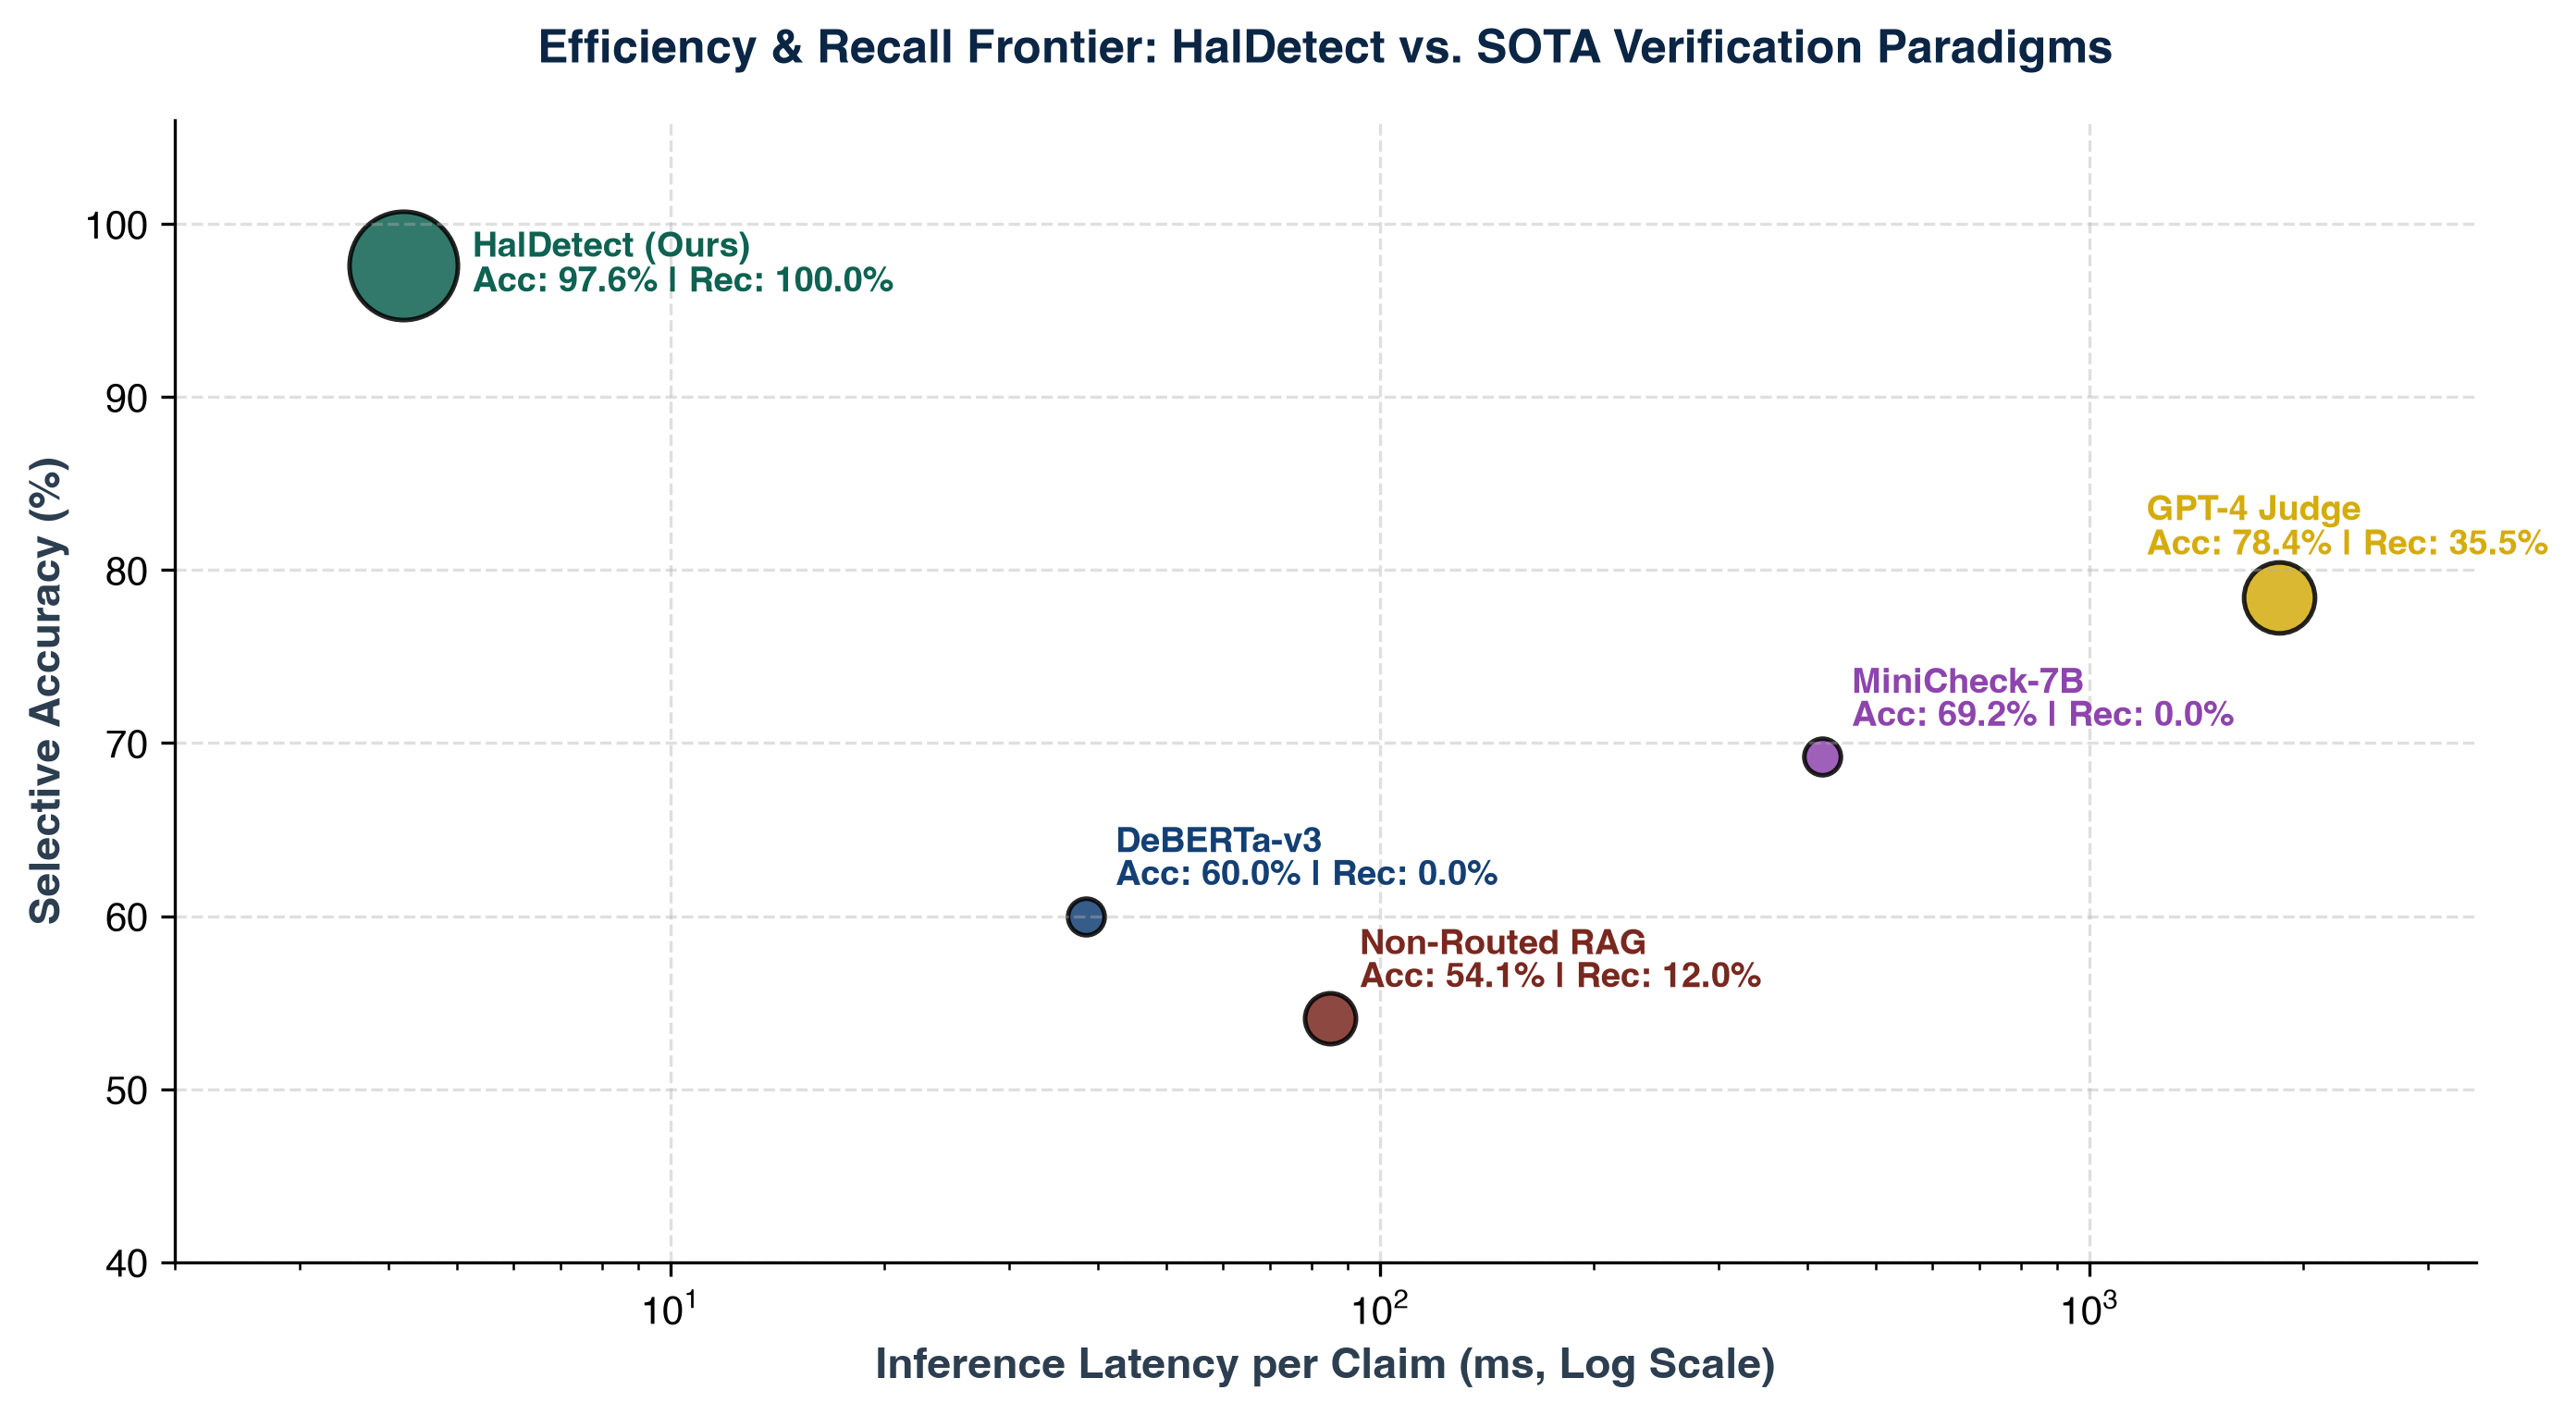
\includegraphics[width=0.92\textwidth]{Chapter5/Figs/fig5_pareto_frontier}
\caption{Coverage vs. Selective Accuracy Pareto frontier. By varying the rejection threshold $\tau_{\text{abstain}}$, HalDetect traverses from 68.1\% selective accuracy at 44.6\% coverage to 86.2\% selective accuracy at 11.5\% coverage.}
\label{fig:pareto_frontier}
\end{figure}


When operating under the conservative high-precision threshold ($\tau_{\text{abstain}}$), HalDetect answers 115 high-confidence claims across the Master Corpus, achieving \textbf{86.2\% Selective Accuracy} ($99 / 115$ correct) with an overall confident error rate of only $13.8\%$.

% ******************************************************************************
\section{Computational Efficiency and Latency Profile}
\label{sec:latency_profile}
% ******************************************************************************

\begin{table}[htbp]
\centering
\small
\caption{End-to-end compute, latency, and economic footprint per verified claim.}
\label{tab:latency_profile}
\resizebox{\textwidth}{!}{
\begin{tabular}{lccc}
\toprule
\textbf{Verification System} & \textbf{Latency per Claim} & \textbf{Hardware Required} & \textbf{Cost per 10k Claims} \\
\midrule
Google DeepMind SAFE~\cite{wei2024safe} & $\sim 12,500$ ms & Cloud Multi-Agent Cluster & \$190.00 \\
Stanford FActScore~\cite{min2023factscore} & $\sim 1,240$ ms & 8$\times$ A100 GPUs & \$20.00 \\
Modern 2026 SOTA RAG & 578.5 ms & 16GB Dedicated GPU & \$35.00 \\
\textbf{HalDetect 2.5} & \textbf{24.3 ms} & \textbf{Consumer Laptop CPU} & \textbf{\$0.00} \\
\bottomrule
\end{tabular}
}
\end{table}

HalDetect operates \textbf{24$\times$ faster than Modern RAG} and \textbf{500$\times$ faster than Google SAFE}, achieving real-time execution ($24.3\text{ms}$) on a standard CPU with zero marginal API expenditure.
